\begin{appendixbox}
        \includegraphics[width=\textwidth]{../Figures/flat/SI1_Human.jpg}
        \captionof{figure}{\textbf{foo}
        \emph{a} test
        } 
        \label{fig:Human}
\end{appendixbox}

\begin{appendixbox}
        \includegraphics[width=\textwidth]{../Figures/flat/SI2_psychometric.jpg}
        \captionof{figure}{\textbf{foo}
        \emph{a} test
        } 
        \label{fig:IndiDiff}
\end{appendixbox}

\begin{appendixbox}
        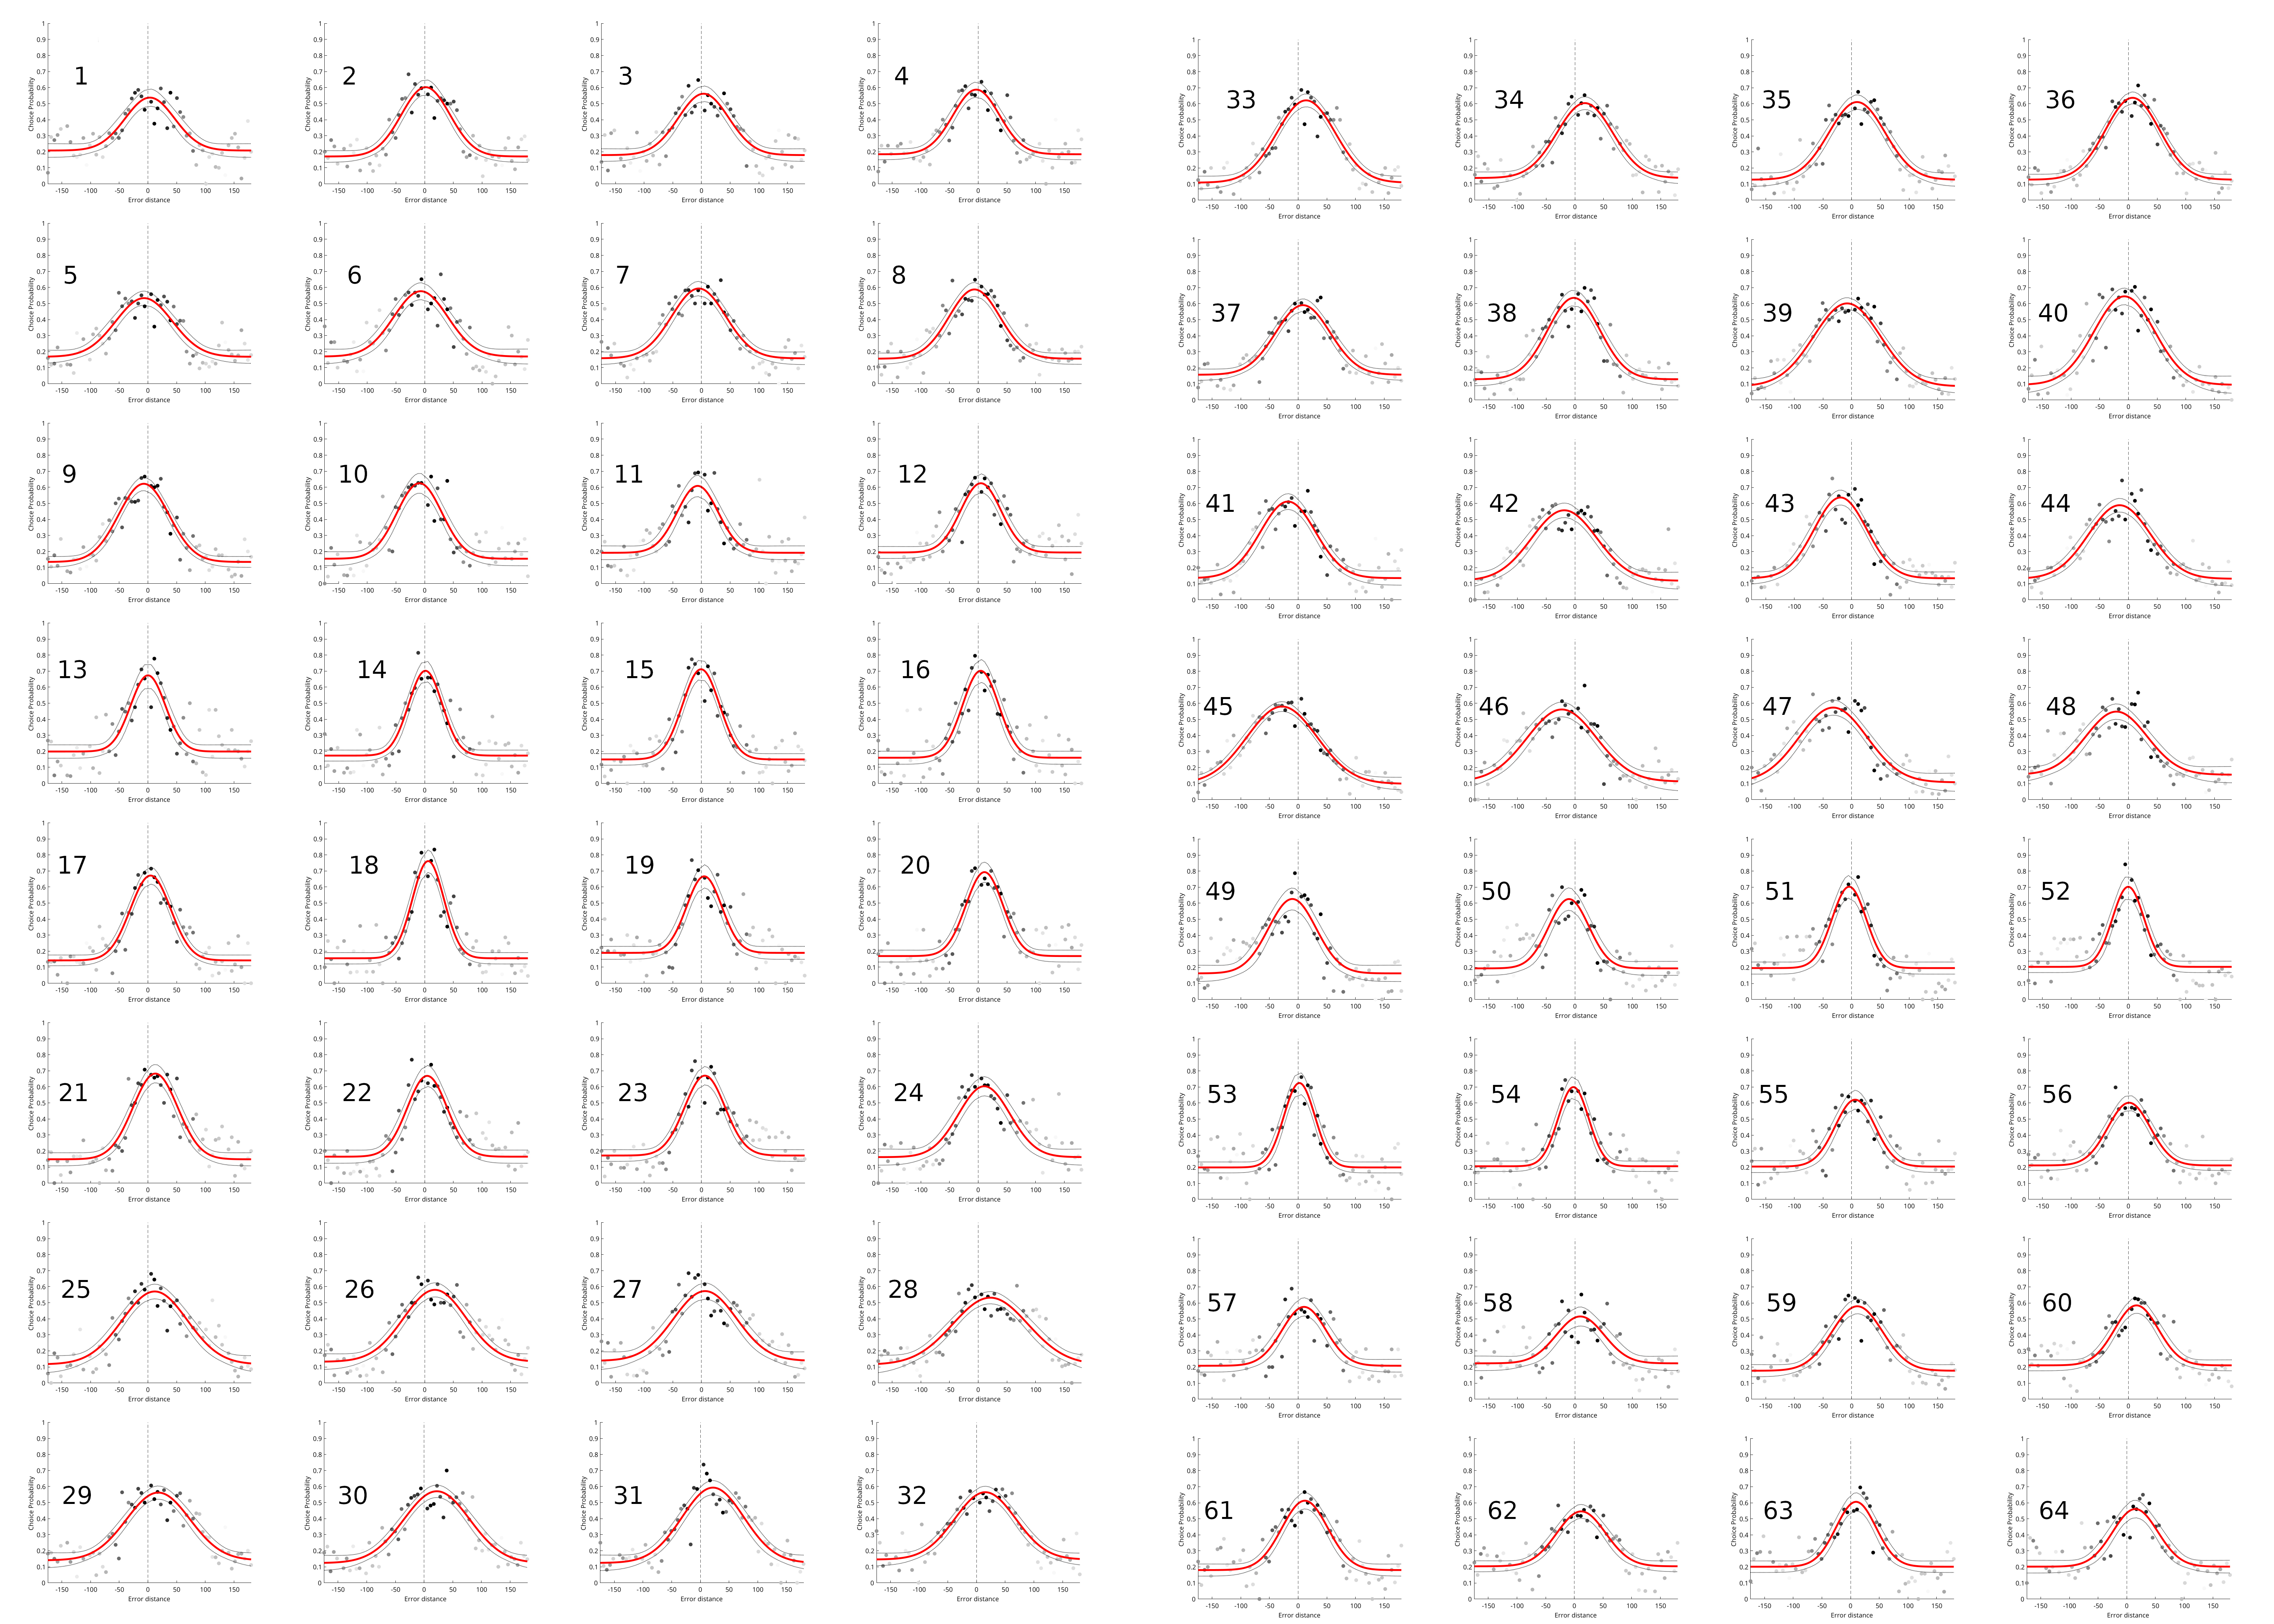
\includegraphics[width=\textwidth]{../Figures/flat/SI3_MMBreakOut.jpg}
        \captionof{figure}{\textbf{foo}
        \emph{a} test
        } 
        \label{fig:MMBreakOut}
\end{appendixbox}

\begin{appendixbox}
        \includegraphics[width=\textwidth]{../Figures/flat/SI4_MM.jpg}
        \captionof{figure}{\textbf{foo}
        \emph{a} test
        } 
        \label{fig:MM}
\end{appendixbox}

\begin{appendixbox}
        \includegraphics[width=\textwidth]{../Figures/flat/SI5_IndTCCv.jpg}
        \captionof{figure}{\textbf{foo}
        \emph{a} test
        } 
        \label{fig:IndiTCC}
\end{appendixbox}

\begin{appendixbox}
        \includegraphics[width=\textwidth]{../Figures/flat/SI6_choiceMatrices.jpg}
        \captionof{figure}{\textbf{foo}
        \emph{a} test
        } 
        \label{fig:choiceProbabilityMatrices}
\end{appendixbox}

